\begin{figure*}
\center{
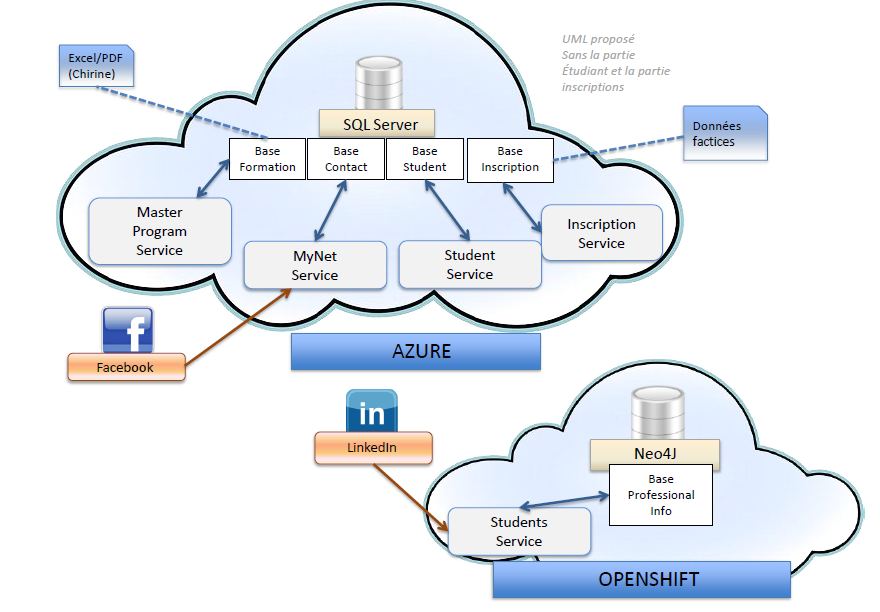
\includegraphics[width=0.65\textwidth]{use-case.png}
\caption{General distributed data storage service.\label{fig:storage}}}
\end{figure*}

Consider a smart city that aims at being energy self-sustainable and produce and consume, as much as possible, energy within its geographic area. 
Producers are characterized according to their location, the amount of energy in Kilowatts-hour that they can sell, the cost of that energy, and the time window in which they can produce it, with a given service level agreement concerning their availability and fault tolerance. 
Consumers are described by their location, their energy requirements during a certain interval of time, the maximum total cost they are ready to pay, and quality of service requirements such as availability and how critical it is to consume this amount of energy. 
An energy exchange market is established in order to continuously trade  energy provision/consumption ensuring that all consumers will have the energy they require at every moment.

In our approach, energy producers are modelled as services with associated ``agreed'' SLAs. 
In general, we assume that several producers will be able to supply energy for a given period of time given specific  preferences expressed by a consumer. 
An energy request is expressed as a query that specifies an energy requirement with QoS preferences independently of the possible producers. 
In our example assume that there are several energy provision services ({\sf e$_1$, ... e$_n$}) that can be independent or hubs integrating several energy providers. 
Each of them is specified by a clause:
\begin{trivlist}\sf\footnotesize
\item[~$\bullet$ ]   e$_i$ $\equiv$ provider(KW-h, Ecost, rate, location), \textit{SLA}$_i$
\end{trivlist}

Services are deployed in different cloud providers and each service exports an agreed SLA that specifies the economic cost per call, the maximum number of calls that can be done per day, the availability of the service, the average response time when a method is called, the reliability, the privacy of the produced data (whether they can be stored or not), the precision, freshness and provenance of the produced data. 
As said in previous sections, some of these measures ({\sf cost/call, maxCall/day}) are static and explicitly specified by the service provider. 
In contrast, the other measures should be computed by monitoring the conversations between the service and the applications that contact it.  
Cloud providers define also their SLA contracts defining normally subscription contracts that specify, the cost per request ({\sf cost/request}), the volume of data that can be exchanged per month ({\sf I/0 volume/month}), the cost of transferring data or applications within the same data centre or between data centres ({\sf datatransferCost/region}), the storage space ({\sf storageSpace}). For example some cloud providers enable the customer to choose the zone to install PaaS services and deploy applications (e.g. zone 1 is Europe). If the customer wishes to deploy services in zone 1 but store data in zone 2 the transfer cost will change.

\begin{trivlist}\sf\footnotesize
\item[~$\bullet$ ] {\sf agreedSLA:$\langle$cost/call, maxCalls/day, availability, responseTime, reliability, privacy, precision, freshness, provenance$\rangle$}. 
 
 \item[~$\bullet$ ]  {\sf cloudSLA:$\langle$cost/request, I/0 volume/month, datatransferCost/region, storageSpace$\rangle$}. 
 \end{trivlist}
 

Queries may be expressed as Datalog-like programs or an SQL-like expressions, including spatio-temporal attributes and preferences.
For instance, \textit{List of energy providers that can provision 1000 Kwatts/h, in the next 10 seconds, that are close to my city with a cost of 0,50 euros/Kwatt and that are labeled as green?}. 
The user preferences statement would include their cloud provider contract and quality preferences:

\begin{trivlist}\sf\footnotesize
\item[~$\bullet$ ]  {\sf cloudSLA:$\langle$0,05 cents per call, 8 Gigabytes I/0 volume/month, free, 1 Giga$\rangle$}. 
\item[~$\bullet$ ] {\sf preferencesStatement:$\langle$query total cost,  total responseTime, reliability, freshness, precision, provenance, storage$\rangle$}. 
\end{trivlist}

We consider a simplified SLA cloud contract inspired in the lowest contract provided by Azure: {\sf cost of \$0,05 cents per call,  8~GB of I/O volume/month, free data transfer cost within the same region,  01~GB of storage}. 
The user is ready to pay maximum {\sf \$5 as total query cost}; she requests that only {\sf green} energy providers are listed (provenance); at least {\sf 85$\%$} of precision of provided data, even if they are not fresh; she requires an availability rate of at least {\sf 90$\%$} and with a response time of {\sf 0,01 seconds}.
 
Assume that there are four household energy providers that can be queried individually and two hubs that collect information from the community smartmeters.
Hubs will store information about (surplus) energy, available from particular users.
We represent these services by {\sf e$_1$, \dots, e$_4$} and {\sf h$_1$ and h$_2$}.
We also suppose the existence of two free location services exporting the following interface: {\sf loc(IP) $\leftarrow$ $\langle$ X, Y$\rangle$}, meaning that given an IP address it returns a geographic position expressed as a pair of coordinates. 
All these services can potentially be combined for answering the query. 
 
 %.  .  .  .  .  . .  .  . .  .  . .  .  . .  .  . .  .  . .  .  . .  .  . .  .  . .  .  . 
 \paragraph{Derived SLA} 
 %.  .  .  .  .  . .  .  . .  .  . .  .  . .  .  . .  .  . .  .  . .  .  . .  .  . .  .  . 
 Some of the user preferences statement measures are used for defining a dervied SLA that, as said in previous section, will guide the evaluation of the query. These measures are defined as a function of the measures used by the agreed SLAs and by the cloud SLA contract.
\begin{trivlist}\sf\footnotesize
\item[~$\bullet$ ] query total cost: $\sum_{i = 1\dots n}$ cost(s$_i$) + data transfer $\leq$ \$5
 \item[~$\bullet$ ] total response time: of services + data transfer
 \item[~$\bullet$ ] availability: {\em (of services involved)} $\leq$ {\sf 90$\%$}, 
 \item[~$\bullet$ ] freshness: non 
 \item[~$\bullet$ ] precision: {\em avg (precision of services involved)} $\leq$ {\sf 85$\%$}
 \item[~$\bullet$ ] provenance:  all services involved must be $green$
 \item[~$\bullet$ ] storage: {\em partial results size} $\leq 1 Giga$ 
 \end{trivlist} 
 
%...---... ...---... ...---... ...---... ...---... ...---... ...---... ...---... ...---... 
  \paragraph{Computing service compositions} 
%...---... ...---... ...---... ...---... ...---... ...---... ...---... ...---... ...---... 

Given a a set of services that can possibly be composed and the derived SLA, a service cmposition must be produced.
Some of the inequations of the derived SLA should be included in the service compositions that answer the query.
In the case of our query example the following composition can be used for answering it:
\begin{eqnarray*}
Q_1 &\equiv&
   \langle X_1,Y_1\rangle = loc_1(IP), \\
&& \langle X_2,Y_2 \rangle = loc_1(Eprovider), \\
&& D = distance(\langle X_1,Y_1\rangle, \langle X_2,Y_2\rangle), \\
&& \langle C_1, E_1 \rangle = e_1(\dots), \dots \langle C_4, E_4 \rangle = e_4(\dots), \\
&& D \leq 1.5 \mathsf{Km},\ \ sum(C_1:C_4) \leq 5, \\
&& sum(E_1:E_4) \geq 1000\ \mathsf{kw-h}, \\
&& \mathsf{totalResponseTime}  \leq 10\ \mathsf{seg}
\end{eqnarray*}

  In fact our approach would generate a number $k$ of service compositions, combining as much as possible the services available such that the constraints of the derived SLA are verified. 
One challenge of this is to generate incremental queries.
 
%.  .  .  .  .  . .  .  . .  .  . .  .  . .  .  . .  .  . .  .  . .  .  . .  .  . .  .  
\paragraph{Optimizing service compositions execution} 
%.  .  .  .  .  . .  .  . .  .  . .  .  . .  .  . .  .  . .  .  . .  .  . .  .  . .  .  .     
A service composition (expressed in a Datalog-like syntax) is then transformed into a query workflow search space consisting of workflows with different control flows and where constraints serve to determine an optimization objective. 
In the case of $Q_1$ above, the corresponding search space contains for example a workflow {\sf QW$_1$} where all activities are executed sequentially. 
Another one, {\sf QW$_2$}, with parallel activities programming the call to a location service for the user and the energy providers, then a filter activity selecting only services located not farther to 1.5 Km, followed by  parallel activities that compute the total cost of the energy to buy, the total amount of energy. 
    
    Once the search space has been computed the QWs are filtered according to their economic and execution time costs. The QWs that minimize this cost are identified and ordered according to their conformance to the user preferences statement.
   
% \begin{figure*}
%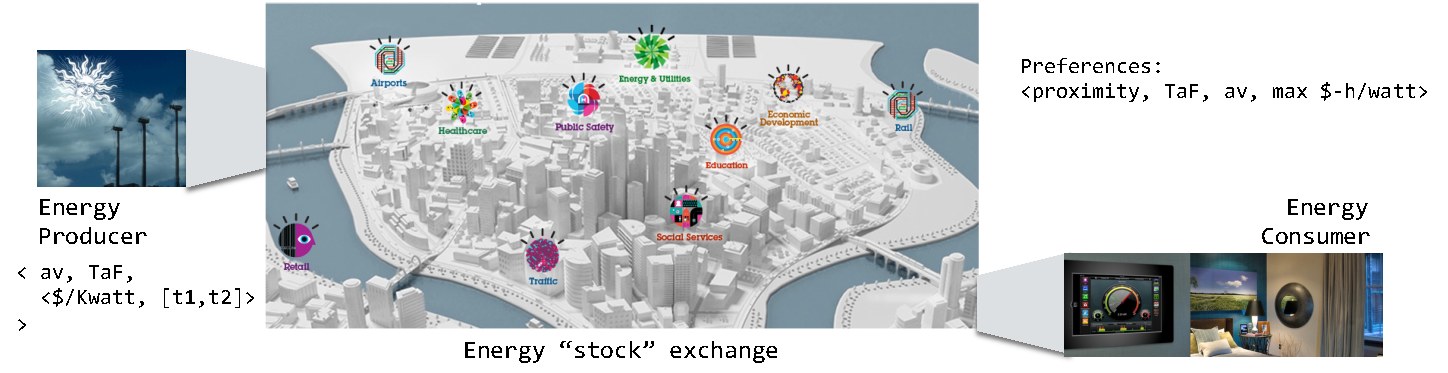
\includegraphics[width=0.95\textwidth]{figs/exchange.pdf}
%\caption{\label{fig:energyXChange} Energy exchange.}
%\end{figure*}